\documentclass[a4paper]{article}

\usepackage[czech]{babel} %https://github.com/michal-h21/biblatex-iso690
\usepackage[
   backend=biber      % if we want unicode 
  ,style=iso-numeric % or iso-numeric for numeric citation method          
  ,babel=other        % to support multiple languages in bibliography
  ,sortlocale=cs_CZ   % locale of main language, it is for sorting
  ,bibencoding=UTF8   % this is necessary only if bibliography file is in different encoding than main document
]{biblatex}

\usepackage[utf8]{inputenc}
\usepackage{fancyhdr}
\usepackage{amsmath}
\usepackage{amssymb}
\usepackage[left=2cm,right=2cm,top=2.5cm,bottom=2.5cm]{geometry}
\usepackage{graphicx}
\usepackage{pdfpages}
\usepackage{url}

\usepackage{siunitx}
\sisetup{locale = DE}  %, separate-uncertainty = true    kdybych chtel +/-

\usepackage{float}
\newfloat{graph}{htbp}{grp}
\floatname{graph}{Graf}
\newfloat{tabulka}{htbp}{tbl}
\floatname{tabulka}{Tabulka}

\renewcommand{\thefootnote}{\roman{footnote}}

\pagestyle{fancy}
\lhead{Praktikum II - (10) Hallův jev}
\rhead{Vladislav Wohlrath}
\author{Vladislav Wohlrath}

\bibliography{source}

\begin{document}

\begin{titlepage}
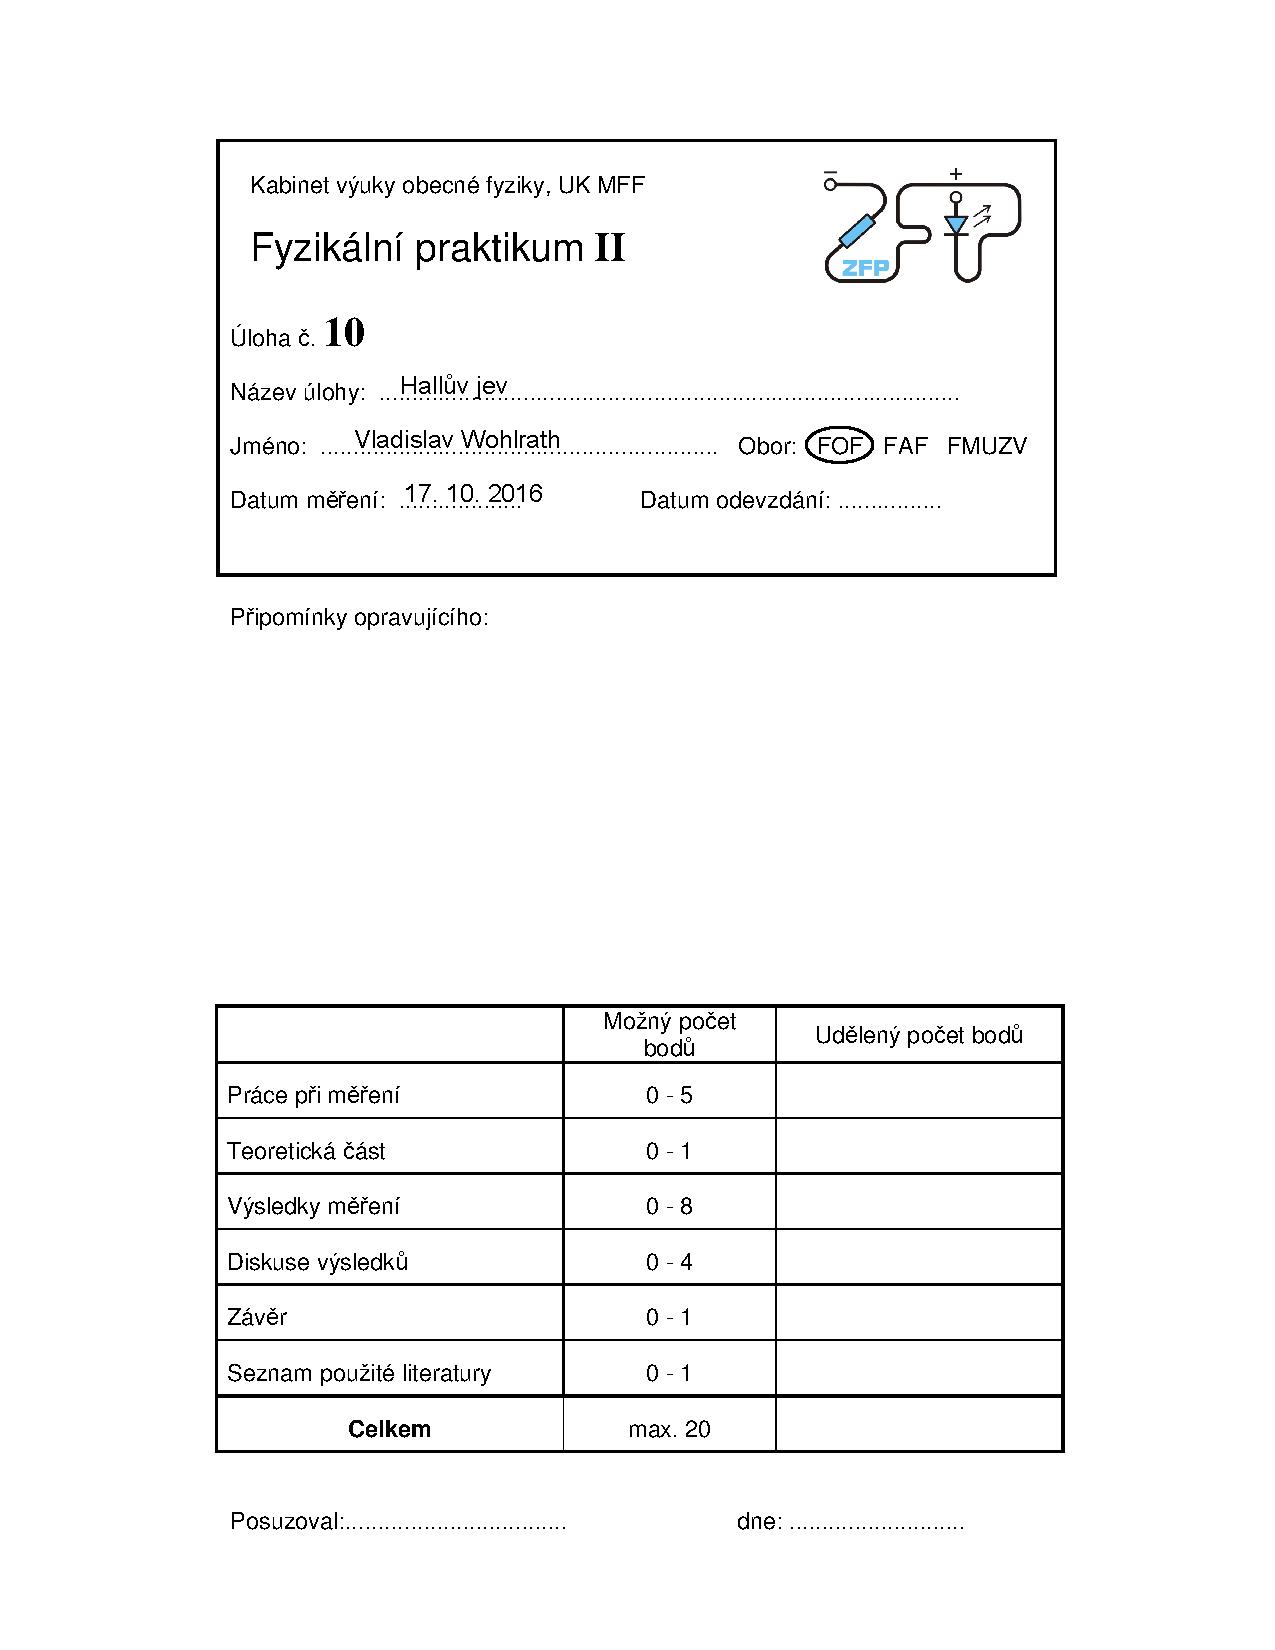
\includepdf[pages={1}]{./graficos/210-tit.pdf}
\end{titlepage}

\section*{Pracovní úkoly}
\begin{enumerate}
\item Zjistěte závislost proudu vzorkem na přiloženém napětí při nulové magnetické indukci.
\item Zjistěte závislost Hallova napětí na magnetické indukci při dvou hodnotách konstantního proudu vzorkem.
\item Výsledky měření zpracujte graficky a vyhodnoťte měrnou vodivost a Hallovu konstantu vzorku.
\item Vypočtěte pohyblivost a koncentraci nositelů náboje.
\end{enumerate}

%Teoretická část
\section*{Teoretická část}

Hlavním cílem této úlohy je změřit pohyblivost $\mu$ a koncentraci $n$ nositelů náboje ve vzorku polovodiče.
Měřený polovodič bude vzorek germania typu n, tedy majoritními nositeli náboje jsou elektrony.
Pohyblivost a koncentraci elektronů určíme ze změřené měrné vodivosti $\sigma$ a Hallovy konstanty $R_H$.

Použitý vzorek je tvaru hranolu s rozměry $t$, $d$ a $l$ a je opatřený šesti kontakty (viz \cite{skripta}).


Měrnou vodivost vzorku určíme z naměřené voltampérové charakteristiky.
Vzorek zapojíme podle schematu \cite{skripta} a naměříme závislost $I_{12}$ na $U_{34}$.
Měrnou vodivost určíme z fitu
\begin{equation} \label{e:vodivost}
I_{12}=\sigma \frac{td}{l} U_{34} \,.
\end{equation}


Pro měření Hallovy konstanty vložíme vzorek procházený proudem $I_{12}$ do pole o magnetické indukci $B$.
V~důsledku působení magnetického pole na pohybující se elektrony ve vzorku se elektrony odchýlí a mezi kontakty 5 a 6 vznikne tzv. Hallovo napětí $U_H$.
Hallovo konstantu určíme z fitu \cite{skripta}
\begin{equation} \label{e:hall}
U_H=R_H\frac{I_{12} \cdot B}{t} \,.
\end{equation}

Vzhledem k tomu, že kontakty 5 a 6 je obtížné umístit přesně symetricky, naměříme na nich při průchodu proudu vzorkem nenulové napětí i při nulové magnetické indukci.
Abychom tento jev eliminovali, změříme napětí při obou polaritách magnetického pole a správnou hodnotu $U_H$ určíme jako
\begin{equation}
| U_H |=|U_{56}^+ - U_{56}^-|/2 \,.
\end{equation}

Mezi $R_H$ a koncentrací $n$ platí vztah \cite{skripta}
\begin{equation} \label{eq:koncentrace}
R_H = \frac{r_H}{en} \,,
\end{equation}
kde $e$ je náboj elektronu a $r_H$ je tzv. rozptylový faktor.
V našem případě můžeme uvažovat $r_H = 3\pi/8$. \cite{skripta}

Ze známé $R_H$ a $\sigma$ můžeme vypočítat tzv. Hallovskou pohyblivost ze vztahu \cite{skripta}
\begin{equation} \label{eq:pohyblivost}
\mu = R_H \sigma \,.
\end{equation}

Magnetické pole budeme realizovat elektromagnetem.

%Podmínky a měřící přístroje
\section*{Podmínky a použité přístroje}

%Výsledky měření
\section*{Výsledky měření}
Měření proběhlo při normálním tlaku a pokojové teplotě (přibližně \SI{22}{\degreeCelsius}).
Všechny uvedené nejistoty jsou standardní a v zápisu \num{10(1)} znamená číslo v závorce nejistotu v řádu poslední uvedené číslice.

Rozměry vzorku byly $l=\SI{6.000(5)}{\mm}$, $d=\SI{3.350(5)}{\mm}$ a $t=\SI{0.720(5)}{\mm}$.




Měrnou vodivost vzorku jsme určili $\sigma = \SI{5.28(5)}{\siemens}$.
Naměřená voltampérová charakteristika je uvedena v tabulce \ref{t:vodivost} a zanesena do grafu \ref{g:vodivost}.


\begin{tabulka}[htbp]
\centering
\begin{tabular}{|cccc|}
\hline 
1 & 2 & 3 & 4 \\
\hline
\end{tabular}
\caption{Voltampérová chrakteristika vzorku}
\label{t:vodivost}
\end{tabulka}

\begin{graph}[htbp] 
\centering
% GNUPLOT: LaTeX picture with Postscript
\begingroup
  \makeatletter
  \providecommand\color[2][]{%
    \GenericError{(gnuplot) \space\space\space\@spaces}{%
      Package color not loaded in conjunction with
      terminal option `colourtext'%
    }{See the gnuplot documentation for explanation.%
    }{Either use 'blacktext' in gnuplot or load the package
      color.sty in LaTeX.}%
    \renewcommand\color[2][]{}%
  }%
  \providecommand\includegraphics[2][]{%
    \GenericError{(gnuplot) \space\space\space\@spaces}{%
      Package graphicx or graphics not loaded%
    }{See the gnuplot documentation for explanation.%
    }{The gnuplot epslatex terminal needs graphicx.sty or graphics.sty.}%
    \renewcommand\includegraphics[2][]{}%
  }%
  \providecommand\rotatebox[2]{#2}%
  \@ifundefined{ifGPcolor}{%
    \newif\ifGPcolor
    \GPcolorfalse
  }{}%
  \@ifundefined{ifGPblacktext}{%
    \newif\ifGPblacktext
    \GPblacktexttrue
  }{}%
  % define a \g@addto@macro without @ in the name:
  \let\gplgaddtomacro\g@addto@macro
  % define empty templates for all commands taking text:
  \gdef\gplbacktext{}%
  \gdef\gplfronttext{}%
  \makeatother
  \ifGPblacktext
    % no textcolor at all
    \def\colorrgb#1{}%
    \def\colorgray#1{}%
  \else
    % gray or color?
    \ifGPcolor
      \def\colorrgb#1{\color[rgb]{#1}}%
      \def\colorgray#1{\color[gray]{#1}}%
      \expandafter\def\csname LTw\endcsname{\color{white}}%
      \expandafter\def\csname LTb\endcsname{\color{black}}%
      \expandafter\def\csname LTa\endcsname{\color{black}}%
      \expandafter\def\csname LT0\endcsname{\color[rgb]{1,0,0}}%
      \expandafter\def\csname LT1\endcsname{\color[rgb]{0,1,0}}%
      \expandafter\def\csname LT2\endcsname{\color[rgb]{0,0,1}}%
      \expandafter\def\csname LT3\endcsname{\color[rgb]{1,0,1}}%
      \expandafter\def\csname LT4\endcsname{\color[rgb]{0,1,1}}%
      \expandafter\def\csname LT5\endcsname{\color[rgb]{1,1,0}}%
      \expandafter\def\csname LT6\endcsname{\color[rgb]{0,0,0}}%
      \expandafter\def\csname LT7\endcsname{\color[rgb]{1,0.3,0}}%
      \expandafter\def\csname LT8\endcsname{\color[rgb]{0.5,0.5,0.5}}%
    \else
      % gray
      \def\colorrgb#1{\color{black}}%
      \def\colorgray#1{\color[gray]{#1}}%
      \expandafter\def\csname LTw\endcsname{\color{white}}%
      \expandafter\def\csname LTb\endcsname{\color{black}}%
      \expandafter\def\csname LTa\endcsname{\color{black}}%
      \expandafter\def\csname LT0\endcsname{\color{black}}%
      \expandafter\def\csname LT1\endcsname{\color{black}}%
      \expandafter\def\csname LT2\endcsname{\color{black}}%
      \expandafter\def\csname LT3\endcsname{\color{black}}%
      \expandafter\def\csname LT4\endcsname{\color{black}}%
      \expandafter\def\csname LT5\endcsname{\color{black}}%
      \expandafter\def\csname LT6\endcsname{\color{black}}%
      \expandafter\def\csname LT7\endcsname{\color{black}}%
      \expandafter\def\csname LT8\endcsname{\color{black}}%
    \fi
  \fi
  \setlength{\unitlength}{0.0500bp}%
  \begin{picture}(10204.00,6802.00)%
    \gplgaddtomacro\gplbacktext{%
      \csname LTb\endcsname%
      \put(682,704){\makebox(0,0)[r]{\strut{} 0}}%
      \csname LTb\endcsname%
      \put(682,1676){\makebox(0,0)[r]{\strut{} 1}}%
      \csname LTb\endcsname%
      \put(682,2648){\makebox(0,0)[r]{\strut{} 2}}%
      \csname LTb\endcsname%
      \put(682,3621){\makebox(0,0)[r]{\strut{} 3}}%
      \csname LTb\endcsname%
      \put(682,4593){\makebox(0,0)[r]{\strut{} 4}}%
      \csname LTb\endcsname%
      \put(682,5565){\makebox(0,0)[r]{\strut{} 5}}%
      \csname LTb\endcsname%
      \put(682,6537){\makebox(0,0)[r]{\strut{} 6}}%
      \csname LTb\endcsname%
      \put(814,484){\makebox(0,0){\strut{} 0}}%
      \csname LTb\endcsname%
      \put(2613,484){\makebox(0,0){\strut{} 0.5}}%
      \csname LTb\endcsname%
      \put(4411,484){\makebox(0,0){\strut{} 1}}%
      \csname LTb\endcsname%
      \put(6210,484){\makebox(0,0){\strut{} 1.5}}%
      \csname LTb\endcsname%
      \put(8008,484){\makebox(0,0){\strut{} 2}}%
      \csname LTb\endcsname%
      \put(9807,484){\makebox(0,0){\strut{} 2.5}}%
      \put(176,3620){\rotatebox{-270}{\makebox(0,0){\strut{}$I_{12}$ (\si{\milli\ampere})}}}%
      \put(5310,154){\makebox(0,0){\strut{}$U_{56}$ (\si{\volt})}}%
    }%
    \gplgaddtomacro\gplfronttext{%
    }%
    \gplbacktext
    \put(0,0){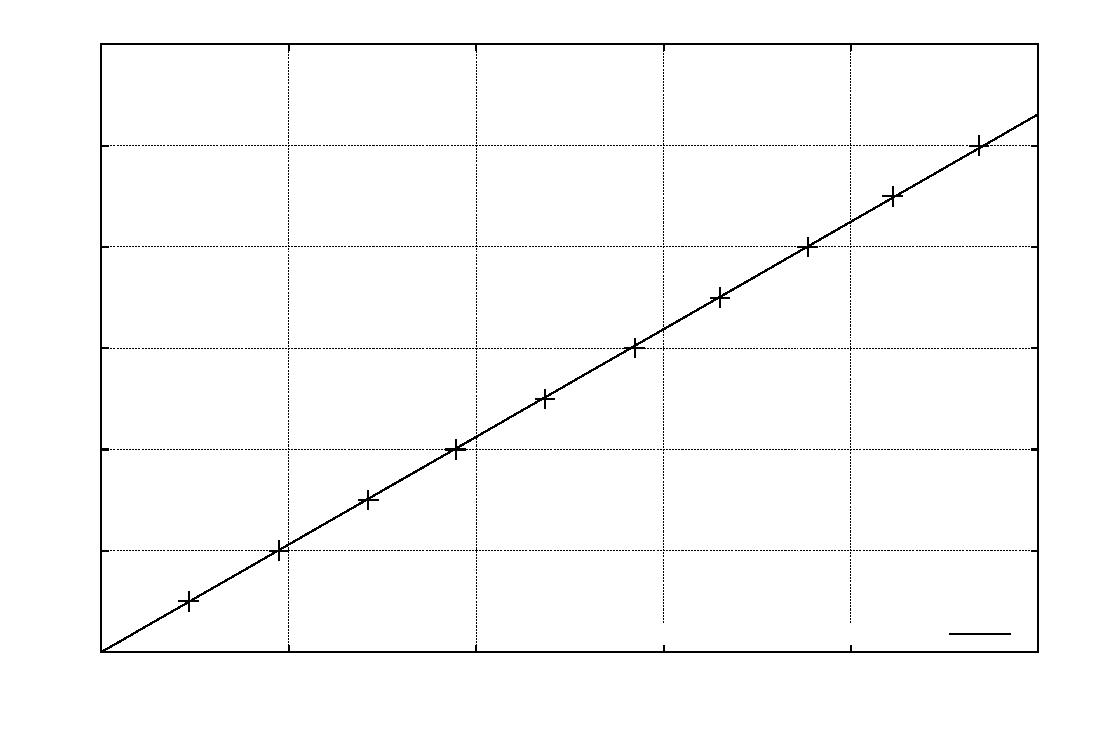
\includegraphics{vod}}%
    \gplfronttext
  \end{picture}%
\endgroup

\caption{Voltampérová charakteristika vzorku}
\label{g:vodivost}
\end{graph}

%Diskuze výsledků
\section*{Diskuze}
Na vzorku jsme zaznamenali parazitické kontaktní napětí, které jsme po konzultaci s vyučujícím vyhodnotili jako ne zcela zanedbatelné. Přesto jsme ho zanedbali.

Naměřené hodnoty vyšly přibližně podle očekávání a řádově jsou jistě správné.

V grafu \ref{g:hall} je vidět, že naměřené hodnoty pro $I_{12}=\SI{2.5}{\milli\volt}$ leží všechny nad proloženou přímkou, zatímco všechny hodnoty pro $I_{12}=\SI{5.0}{\milli\volt}$ leží pod ní.
Přesná přícina je nám neznámá, možné vysvětlení je, že jeden z parametrů $\mu$ nebo $n$ není zcela nezávislý na procházejícím proudu a tedy i $R_H$ je pro různé proudy jiné.
Naměřené hodnoty pro oba proudy $I_{12}$ ale přibližně odpovídají teoretické závislosti a má proto smysl uvažovat pouze jednu hodnotu $R_H$.

%Závěr
\section*{Závěr}
Změřili jsme měrnou vodivost vzorku $\sigma = \SI{5.28(5)}{\siemens\per\meter}$ a Hallovu konstantu $R_H = \SI{0.061(1)}{\meter\cubed\per\ampere\per\second}$.

Pomocí těchto údajů jsme určili Hallovskou pohyblivost elektronů ve vzorku $\mu = \SI{0.324(3)}{\ampere\metre\squared\per\kg}$ a jejich koncentraci $n = \num{1.07(1)} \cdot \SI{e20}{\per\metre\cubed}$.


\printbibliography[title={Seznam použité literatury}]

\end{document}